\chapter{Use Cases} \label{use-cases} % Yutong / Jake [DONE]

The two actors involved are users and developers. Each of their respective functions are listed in Figure~\ref{fig:use-cases}.

\section{User Use Cases}
The users can play the game from both their own perspective, which will be interacting with a virtual child, and the child's perspective. The users can also keep track of their personal progress by checking out the report generated.

\begin{table}[!ht]
\centering
\caption{Play as Parent Use Case}
\label{table:game-as-parent}
\vspace{5mm}
\resizebox{0.66\textwidth}{!}{%
\begin{tabular}{@{}l|lllll@{}}
\toprule
\textbf{Use Case Name}      & Play as parent \\
\midrule
\textbf{Goal}               & Interact with virtual child \\ 
\midrule
\textbf{Actor(s)}           & User \\
\midrule
\textbf{Precondition(s)}    & Be logged in as User \\
\midrule
\textbf{Postcondition(s)}   & VR child is happy \\
\midrule
\textbf{Exception(s)}       & N/A \\
\midrule
\end{tabular}%
}
\end{table}

\begin{table}[!ht]
\centering
\caption{Play as Child Use Case}
\label{table:game-as-child}
\vspace{5mm}
\resizebox{0.66\textwidth}{!}{%
\begin{tabular}{@{}l|lllll@{}}
\toprule
\textbf{Use Case Name}      & Play as child \\
\midrule
\textbf{Goal}               & Empathize with child\\ 
\midrule
\textbf{Actor(s)}           & User \\
\midrule
\textbf{Precondition(s)}    & Be logged in as User \\
\midrule
\textbf{Postcondition(s)}   & Experienced child's perspective \\ 
\midrule
\textbf{Exception(s)}       & N/A \\
\midrule
\end{tabular}%
}
\end{table}

\begin{table}[!ht]
\centering
\caption{Track Personal Progress Use Case}
\label{table:track-progress}
\vspace{5mm}
\resizebox{0.66\textwidth}{!}{%
\begin{tabular}{@{}l|lllll@{}}
\toprule
\textbf{Use Case Name}      & Track personal progress \\
\midrule
\textbf{Goal}               & View and learn from progress\\ 
\midrule
\textbf{Actor(s)}           & User \\
\midrule
\textbf{Precondition(s)}    & Be logged in as User \\
\midrule
\textbf{Postcondition(s)}   & Display historical data\\
\midrule
\textbf{Exception(s)}       & N/A \\
\midrule
\end{tabular}%
}
\end{table}

\clearpage

\section{Developer Use Cases}

With the system, the developers are able to develop personalize "training plan" based on the user data, while the users can play game and keep track of their personal progress. The developers can decide the stress level for the user by analyzing the collected user data. While measuring the current stress level of the user, the developers can adjust then the difficulty of the game based on the user's stress level in real time.


\begin{table}[!ht]
\centering
\caption{Collect User Data Use Case}
\label{table:collect-data}
\vspace{5mm}
\resizebox{0.66\textwidth}{!}{%
\begin{tabular}{@{}l|lllll@{}}
\toprule
\textbf{Use Case Name}      & Collect user data \\
\midrule
\textbf{Goal}               & Track user progress\\ 
\midrule
\textbf{Actor(s)}           & Developer \\
\midrule
\textbf{Precondition(s)}    & Be logged in as Developer \\
\midrule
\textbf{Postcondition(s)}   & User data sent to be analyzed \\
\midrule
\textbf{Exception(s)}       & N/A \\
\midrule
\end{tabular}%
}
\end{table}

\begin{table}[!ht]
\centering
\caption{Analyze User Data Use Case}
\label{table:analyze-data}
\vspace{5mm}
\resizebox{0.66\textwidth}{!}{%
\begin{tabular}{@{}l|lllll@{}}
\toprule
\textbf{Use Case Name}      & Analyze user data \\
\midrule
\textbf{Goal}               & Study user progress\\ 
\midrule
\textbf{Actor(s)}           & Developer \\
\midrule
\textbf{Precondition(s)}    & Be logged in as Developer \\
\midrule
\textbf{Postcondition(s)}   & Analysis stored in centralized location \\
\midrule
\textbf{Exception(s)}       & N/A \\
\midrule
\end{tabular}%
}
\end{table}

\begin{table}[!ht]
\centering
\caption{Decide Stress Level Use Case}
\label{table:decide-stress}
\vspace{5mm}
\resizebox{0.66\textwidth}{!}{%
\begin{tabular}{@{}l|lllll@{}}
\toprule
\textbf{Use Case Name}      & Decide stress level \\
\midrule
\textbf{Goal}               & Adjust game intensity\\ 
\midrule
\textbf{Actor(s)}           & Developer \\
\midrule
\textbf{Precondition(s)}    & Be logged in as Developer \\
\midrule
\textbf{Postcondition(s)}   & Stress levels calculated \\
\midrule
\textbf{Exception(s)}       & N/A \\
\midrule
\end{tabular}%
}
\end{table}

\begin{table}[!ht]
\centering
\caption{Measure Current Stress level Use Case}
\label{table:measure-stress}
\vspace{5mm}
\resizebox{0.66\textwidth}{!}{%
\begin{tabular}{@{}l|lllll@{}}
\toprule
\textbf{Use Case Name}      & Measure current stress level \\
\midrule
\textbf{Goal}               & Track historical stress data\\ 
\midrule
\textbf{Actor(s)}           & Developer \\
\midrule
\textbf{Precondition(s)}    & Be logged in as Developer \\
\midrule
\textbf{Postcondition(s)}   & Heart rate readings stored in centralized location \\
\midrule
\textbf{Exception(s)}       & N/A \\
\midrule
\end{tabular}%
}
\end{table}

\begin{table}[!ht]
\centering
\caption{Adjust Game Difficulty Use Case}
\label{table:game-with-child}
\vspace{5mm}
\resizebox{0.66\textwidth}{!}{%
\begin{tabular}{@{}l|lllll@{}}
\toprule
\textbf{Use Case Name}      & Adjust game difficulty \\
\midrule
\textbf{Goal}               & Personalize user experience\\ 
\midrule
\textbf{Actor(s)}           & Developer \\
\midrule
\textbf{Precondition(s)}    & Be logged in as Developer \\
\midrule
\textbf{Postcondition(s)}   & Difficulty reflects user stress\\
\midrule
\textbf{Exception(s)}       & N/A \\
\midrule
\end{tabular}%
}
\end{table}

\begin{table}[!ht]
\centering
\caption{Generate Report Use Case}
\label{table:generate-report}
\vspace{5mm}
\resizebox{0.66\textwidth}{!}{%
\begin{tabular}{@{}l|lllll@{}}
\toprule
\textbf{Use Case Name}      & Generate report \\
\midrule
\textbf{Goal}               & Record user progress\\ 
\midrule
\textbf{Actor(s)}           & Developer \\
\midrule
\textbf{Precondition(s)}    & Be logged in as Developer \\
\midrule
\textbf{Postcondition(s)}   & Report is sent to user \\
\midrule
\textbf{Exception(s)}       & N/A \\
\midrule
\end{tabular}%
}
\end{table}

\begin{figure}[!ht]
    \centering
    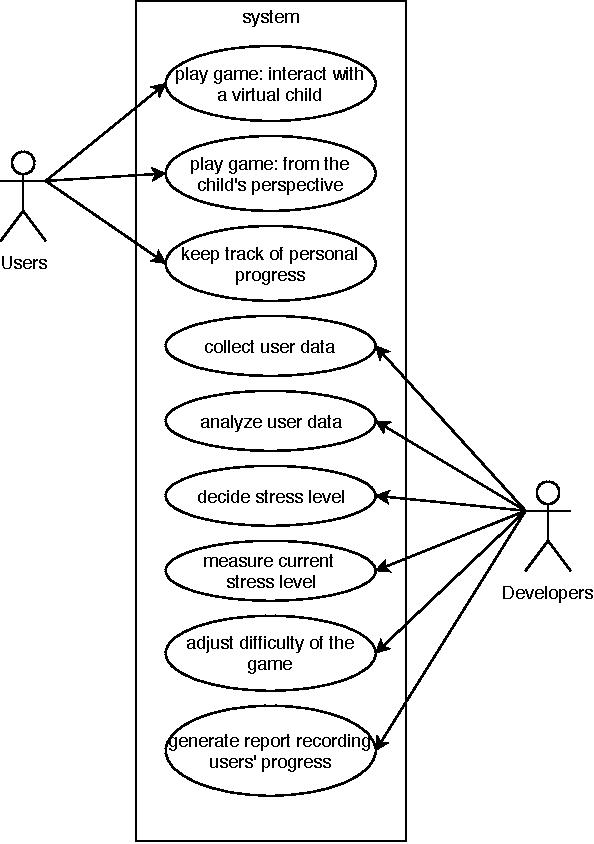
\includegraphics[width=0.6\linewidth]{use-cases}
    \caption{Use Cases}
    \label{fig:use-cases}
\end{figure}




